\chapter{Resultaten met het ingebouwd model}
\label{ch:resultaten-ingebouwd-model}

De 845 beelden van Huis van Alijn werden getagged door het general model van Clarifai. Aan iedere foto werden twintig tags gegeven. De waarschijnlijkheidsscore van de tags bevond zich tussen 100\% en 65\% en had een gemiddelde van 93\%. 

De verkregen tags zijn op te delen in een aantal categorieën en gaan over verschillende aspecten van het beeld:
\begin{itemize}
	\item entiteiten die op de beelden te zien zijn, waaronder \textit{volwassene}, \textit{speelgoed}, \textit{bloem}, \textit{kameel}, \textit{jurk}, \textit{meubels} en \textit{strand};
	\item activiteiten die uitgevoerd worden op de beelden, zoals \textit{dansen}, \textit{zitten}, \textit{rusten}, \textit{shoppen} en \textit{reizen};
	\item emoties of gevoelens die te zien zijn op het beeld of die opgeroepen worden door het beeld, denk aan \textit{plezier}, \textit{liefde}, \textit{genot}, \textit{avontuur}, \textit{affectie}, \textit{sexy} en \textit{mooi};
	\item maar ook contextuele concepten, zoals \textit{vriendschap}, \textit{familie}, \textit{toerisme}, \textit{vrije tijd} en \textit{het samen zijn};
	\item en hoeveelheden: \textit{één}, \textit{twee}, \textit{drie}, \textit{vier}, \textit{veel}, \textit{enkele}. Dit waren vaak weinigzeggende termen die opvallend vaak fout waren. Het was ook niet altijd duidelijk waar die hoeveelheden op sloegen. Veel mensen? Veel bloemen?
	\item tot slot kregen we ook informatie over de foto zelf: \textit{portret}, \textit{kleur}, \textit{zwart-wit}, \textit{sepia}, \textit{monochroom}...
\end{itemize}

Tijdens de validatie werd vastgesteld dat Clarifai veel algemene termen geeft, zoals \textit{mensen}, \textit{volwassene}, \textit{kind}, \textit{groep} en \textit{veel}, maar soms waren we ook verwonderd over de relevantie van de tags. Enkele van die relevante tags zijn: \textit{schildersezel}, \textit{roos}, \textit{uitstapje}, \textit{airbus}, \textit{souvenir}, \textit{bazaar}, \textit{grasland}, \textit{broche} en \textit{bruidsmeisje}. 

Na validatie bleken 11.517 van de 16.900 tags correct te zijn (68,15\%). Dit resulteerde in 371 unieke termen die de foto’s beschreven. Bij 21 foto’s waren alle twintig tags correct. 97 beelden (11,5\%) hadden minder dan tien correcte tags, waarvan de slechts scorende een foto is van het thema speelgoed. Deze foto had slechts zes juiste tags. Gemiddeld hadden de foto’s 13,6 correcte tags.

\begin{figure}
	%TODO slechte foto toevoegen
	\centering
	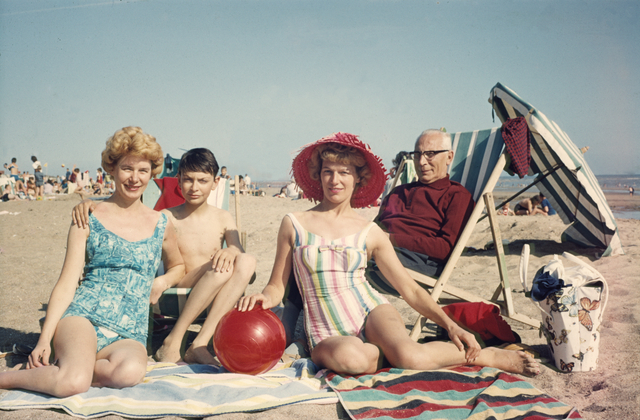
\includegraphics[width=0.495\textwidth]{DIA-0078-0352.jpg}\hfill
	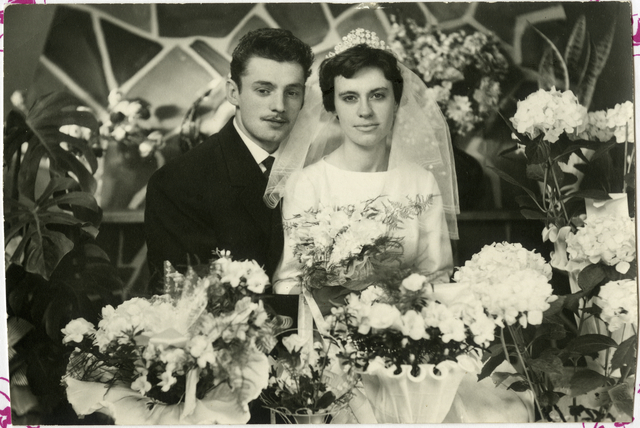
\includegraphics[width=0.495\textwidth]{FO-50-01658.jpg}\hfill
	\\[\smallskipamount]
	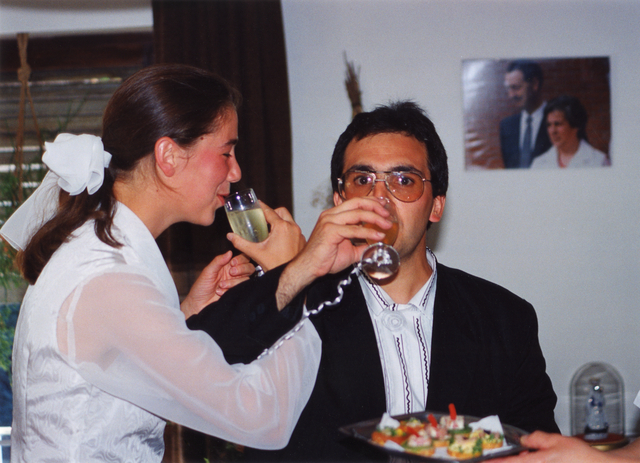
\includegraphics[width=0.495\textwidth]{FO-90-00157.jpg}\hfill
	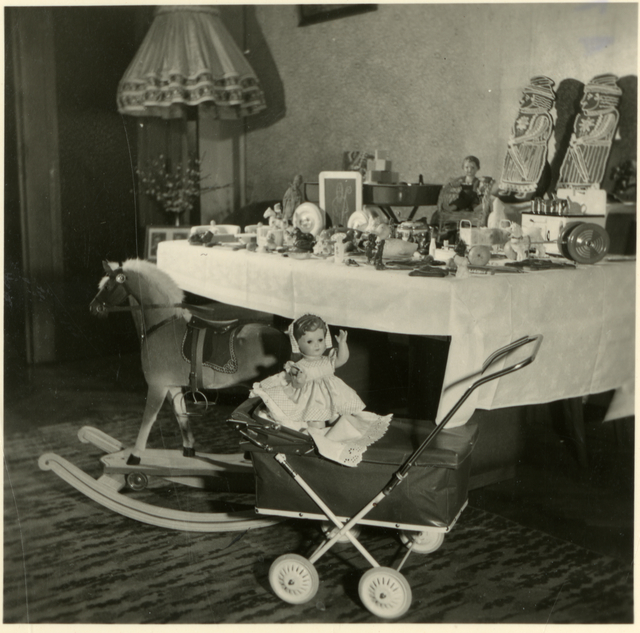
\includegraphics[width=0.495\textwidth]{FO-50-02073.jpg}\hfill
	\caption[Enkele voorbeelden van foto's die goed of slecht getagged werden door het ingbouwde Clarifai-model]{Drie foto’s uit de fotocollectie van Huis van Alijn waarvan alle tags correct waren en de foto waar het minst aantal tags correct waren (rechtsonder).}
\end{figure}

Vooraf hadden we verwacht dat het model niet goed zou scoren op de Sinterklaasfoto’s. Sinterklaas is immers een ritueel dat enkel voorkomt in de lage landen en enkele vroegere koloniën van Nederland. De kans lijkt dus klein dat het model de concepten van Sinterklaas kent. Omdat modellen voornamelijk getraind worden met hedendaagse foto’s, vreesden we ook dat de resultaten met de oudere foto’s minder goed zouden zijn.

%TODO referenties naar tabellen
Na validatie bleek het vermoeden rond de Sinterklaasfoto’s correct te zijn (zie tabel). Het valt meteen op dat dit thema het laagste gemiddelde en het hoogst aantal foto’s met minder dan tien correcte tags heeft. Aan de beelden van dit thema werden tevens het minst aantal unieke termen gegeven. Het model blijkt ook minder goed op het speelgoedthema te scoren. De resultaten voor de huwelijksfoto’s zijn dan weer erg goed. Het gemiddelde voor dit thema is ongeveer 1,5 punten beter dan het gemiddelde van alle beelden.

%TODO tabellen invoegen

%TODO referenties naar tabel
Wat betreft de periodes is het moeilijker om conclusies te trekken. Uit tabelkan afgeleid worden dat de recentere foto’s (1960-1999) beter scoren en dat de oudste foto’s het slechts scoren. Niettemin moet hier nuance van gemaakt worden. Er zijn immers slechts negen beelden uit de jaren 1900. Bovendien bestaan foto’s uit de jaren 50 - en in mindere mate uit de jaren 40 - voor een groot deel uit foto’s over Sinterklaas, wat hun slechtere score kan verklaren. Foto’s uit de jaren 60 scoren opmerkelijk goed, maar dit valt dan weer te verklaren door de grote aanwezigheid van huwelijksfoto’s in die periode (meer dan 75\%).\footnote{zie \ref{sec:analyseren-van-de-dataset}}

\section{Gedetailleerde resultaten per thema}
\label{sec:gedetailleerde-resultaten-per-thema}

In dit deel wordt dieper ingegaan op de resultaten per thema. Voor ieder thema wordt de top 30 van meest voorkomende termen, het maximale, minimale en gemiddeld aantal correcte tags, het aantal beelden met minder dan tien juiste tags en het aantal unieke termen toegelicht. 

\subsection{Geboorte}

In totaal waren er 96 beelden voor dit thema. De API scoorde goed op deze foto’s, in lijn met het totale gemiddelde. Er werden 112 unieke termen gebruikt om de beelden te beschrijven. Gemiddeld waren 13,7 tags correct. Het maximale aantal correcte tags was twintig, het minste zeven. Slechts zeven beelden hadden minder dan tien correcte tags (7,2\%).

\begin{figure}
	%TODO slechte foto toevoegen
	\centering
	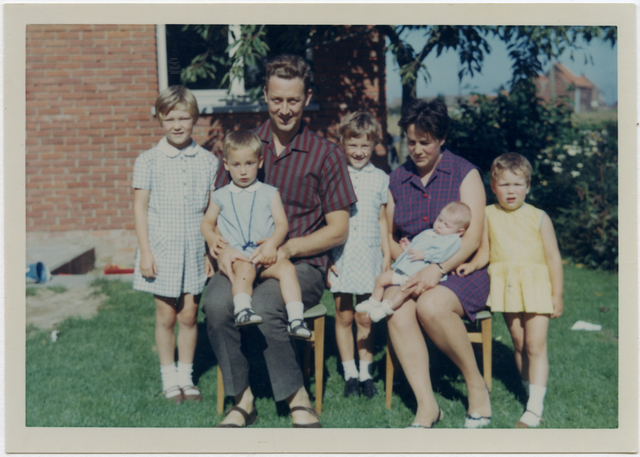
\includegraphics[width=0.495\textwidth]{FO-60-01055.jpg}\hfill
	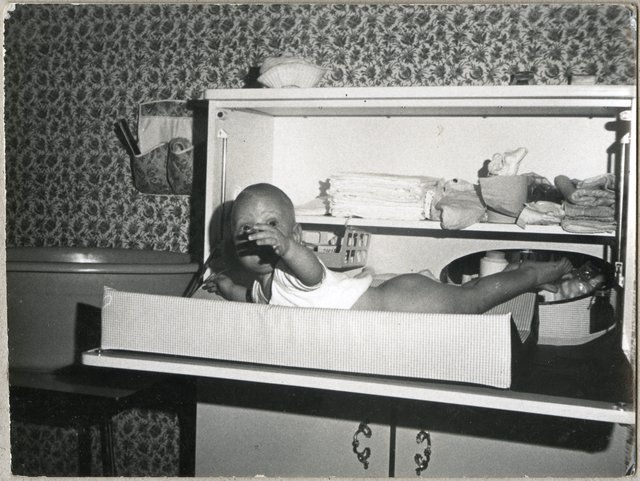
\includegraphics[width=0.495\textwidth]{FO-70-00900.jpg}\hfill
	\caption[Best en slechtst scorende foto van thema geboorte]{een best scorende (links) en slechtst scorende (rechts) foto van het thema geboorte uit de fotocollectie van het Huis van Alijn.}
\end{figure}

De dertig meest voorkomende termen verwijzen naar mensen, kinderen en nakomelingen. Het model ziet ook enkele emoties in de beelden: liefde en affectie. Het merendeel van de foto’s waren ook portretten van moeder (en soms ook vader) met baby. Soms stonden er ook andere mensen, zoals broers, zussen, familieleden en vrienden op de foto. 

Uit de top 30 valt op dat er een groot verschil is tussen het aantal verschijningen van de meest voorkomende term (93 keer) en die op plaats 30 (7 keer). De top 11 komt in minstens de helft van de beelden voor. Het valt hierbij ook op dat term baby slechts aan de helft van de foto’s gegeven is.

\begin{table}
	\centering
	\begin{tabular}{*{3}{l}}
		mensen (93) & zoon (48) & gezichtsexpressie (22) \\
		volwassene (83) & 	groep (35) & meisje (19) \\
		kind (82) & twee (32) & affectie (17) \\
		vrouw (76) & sepia (29) & drie (16) \\
		portret (75) & binnenshuis (27) & verschillende (15) \\
		familie (65) & 	kamer (27) & broer of zus (13) \\
		kledij (62) & 	meubels (25) & bed (10) \\
		nageslacht (51) & liefde (25) & jongen (8) \\
		man (49) & samenkomen (24) & voertuig (7) \\
		baby (48) & monochroom (23) & stoel (7) \\	
	\end{tabular}
	\caption{De dertig meest voorkomende tags van geboortefoto's met het ingebouwde Clarifai-model}
	\label{tab:30-termen-geboorte}
\end{table}

Een opvallende vaststelling was dat het model de term \textit{dochter} niet kent; enkel \textit{zoon} werd gegeven. Doordat het voor ons niet mogelijk was om het verschil tussen een mannelijke en een vrouwelijke baby te zien, hebben we dit altijd als correct beschouwd.

Het model vergiste zich soms ook. Man en vrouw met kind werden in zestien van de gevallen door het model als een trouwfoto beschouwd. Ook de tags bruidegom (3 keer) en bruid kwamen voor (2 keer). Dit is vermoedelijk doordat op die foto’s de baby gewikkeld was in een sluier, wat verkeerdelijk door het model als een bruidssluier gepercipieerd werd.